\documentclass[varwidth=true, border=2pt]{standalone}
\usepackage{tikz}
\begin{document}

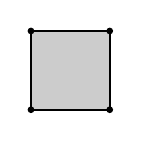
\begin{tikzpicture}[line join=bevel,z=-5.5]
    \coordinate (0) at (0,0);
    \coordinate (1) at (1,0);
    \coordinate (2) at (1,1);
    \coordinate (3) at (0,1);


%   \draw  -- (B1) -- cycle;
%\draw (A4) -- (A1) -- (B1) -- cycle;
    \fill[black!20!white] (0) -- (1) -- (2) -- (3) -- cycle;
    \draw[fill=black] (0,0) circle (1pt);
    \draw[fill=black] (1,0) circle (1pt);
    \draw[fill=black] (1,1) circle (1pt);
    \draw[fill=black] (0,1) circle (1pt);
    \draw[thick] (0,0) -- (1,0);
    \draw[thick] (1,0) -- (1,1);
    \draw[thick] (1,1) -- (0,1);
    \draw[thick] (0,1) -- (0,0);
\end{tikzpicture}

\end{document}